% latex uft-8
\documentclass[uplatex,a4paper,11pt,oneside,openany]{jsarticle}
%
\usepackage[T1]{fontenc}
\usepackage[dvipdfmx]{graphicx}
\usepackage[dvipdfmx]{color}
\usepackage{amsmath,amssymb}
\usepackage{enumerate}
\usepackage{bm}
\usepackage{graphicx}
\usepackage{ascmac}
\usepackage{setspace}
\usepackage{here}
\usepackage{url}
\usepackage{ulem}
\usepackage{colortbl}
\usepackage{comment}
\usepackage{setspace}
\usepackage{multicol}
\usepackage{multicolpar}
\usepackage{listings,jlisting} %日本語のコメントアウトをする場合jlistingが必要
%ここからソースコードの表示に関する設定
\lstset{
	%プログラム言語(複数の言語に対応,C,C++も可)
	language = Python,
	%背景色と透過度
	backgroundcolor = {\color[gray]{.95}},
	%枠外に行った時の自動改行
	breaklines = true,
	%自動改行後のインデント量(デフォルトでは20[pt])
	breakindent = 10pt,
	%標準の書体
	%basicstyle = \ttfamily\scriptsize,
	basicstyle = \fontsize{8}{10}\selectfont\ttfamily,
	%コメントの書体
	commentstyle = {\itshape \color[cmyk]{1,0.4,1,0}},
	%関数名等の色の設定
	classoffset = 0,
	%キーワード(int, ifなど)の書体
	keywordstyle = {\bfseries \color[cmyk]{0,1,0,0}},
	%表示する文字の書体
	stringstyle = {\ttfamily \color[rgb]{0,0,1}},
	%枠 "t"は上に線を記載,"T"は上に二重線を記載
	%他オプション:leftline,topline,bottomline,lines,single,shadowbox
	frame = TBrl,
	%frameまでの間隔(行番号とプログラムの間)
	framesep = 5pt,
	%行番号の位置
	numbers = left,
	%行番号の間隔
	stepnumber = 1,
	%行番号の書体
	numberstyle = \tiny,
	%タブの大きさ
	tabsize = 4,
	%キャプションの場所("tb"ならば上下両方に記載)
	captionpos = t
}
%ここまでソースコードの表示に関する設定

\begin{document}
	\title{C言語:オセロ(リバーシ)}
	\author{◯×工業高校 機械工学科 2年}
	\date{\today}
	\maketitle
	\pagestyle{empty}

%\newpage
	
\section{ゲームの概要}

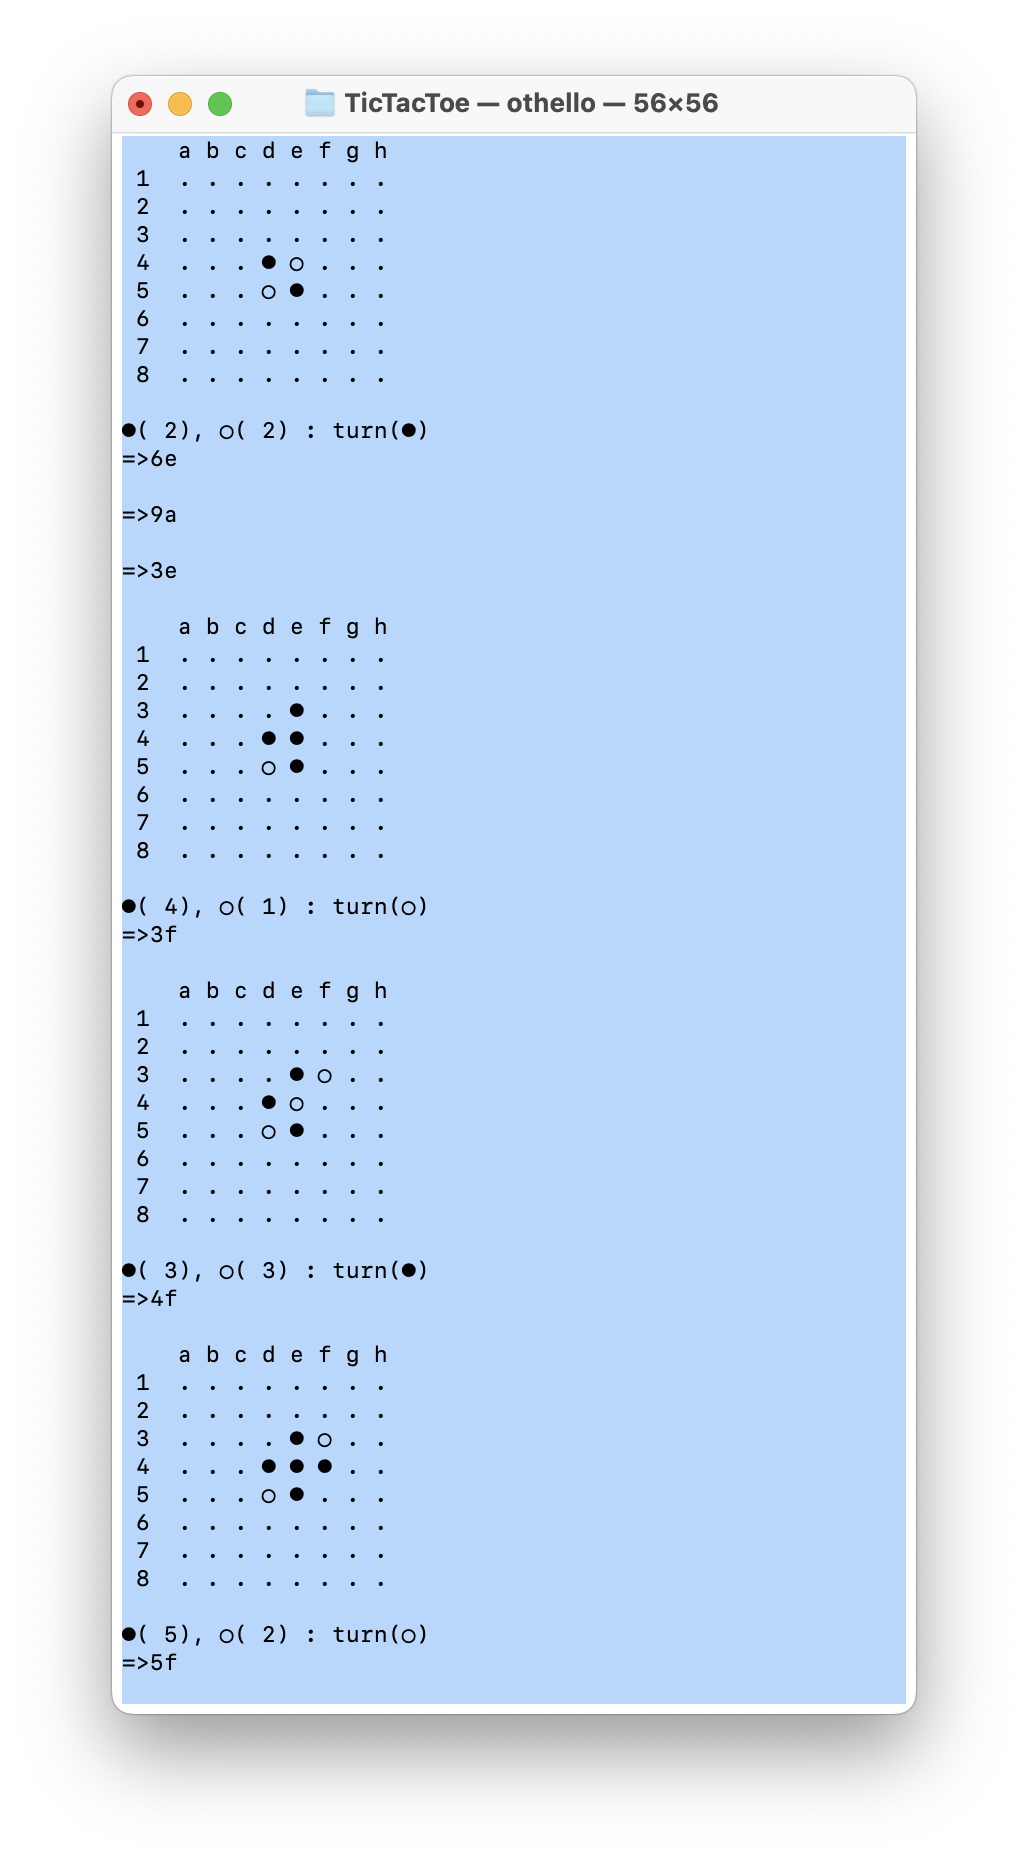
\includegraphics[keepaspectratio,scale=0.5]{othelloview.png}

\newpage

\section{各種宣言など}

\begin{enumerate}
\item これは冒頭に記述する
\item BOOLEAN形を enum で定義する
\item 盤面の幅BOARDWは \#define 文で指定する
%それは$4 \times 4, 6 \times 6, 8 \times 8$など、4以上8以下の偶数でなければならない
\item 盤面に黒の石が置かれている場所にはBLACK 、白の石が置かれている場所はWHITE、何も置かれていない場所はNONEで区別する
\item 現在注目している石の位置(x,y)から見て、下の方向には(0,-1)、右下には(1,-1)、右には(0,1)、右上には(1,1)、上には(1,0)、左上には(-1,1)、左には(-1,0)、左下には(-1,-1)を加えることで、上下、左右、斜め右上下、斜め左上下の、全部で8つの方向の場所を確認していくことができる
\item 盤面上の場所(x,y)を指定するための構造体POSを定義する
\item 盤面状態を保持している1次元配列board上の位置は、POS型変数(x,y)から\\$y \times BOARDW +x$によって求める
\item 手番は変数turnに保持している
\item パスの回数passcountが2回になるとゲームは終了する
\item 終了フラグendglagが偽である間ゲームは続く
\item setstone()関数は盤面の指定位置に石を置く操作
\item getstone()関数は盤面の指定位置の状態を知る操作
\end{enumerate}

\begin{lstlisting}
	#include <stdio.h>
	#include <stdlib.h>
	
	enum BOOLEAN{
		false,    /* false=0, true=1 */
		true
	};
	
	#define BOARDW (8) // 4, 6, 8, ....
	#define BLACK (0)
	#define WHITE (1)
	#define NONE (2)
	
	int UNITV[][2] = {{0,-1},{1,-1},{1,0},{1,1},{0,1},{-1,1},{-1,0},{-1,-1}};
	int turn = BLACK;
	int passcount = 0;
	int endflag = false;
	int board[BOARDW * BOARDW];
	
	const char* TILE[] = {
		"●",  //TILE_BLACK
		"◯",  //TILE_WHITE
		"."   //TILE_NONE
	};
	
	typedef struct {
		int x, y;
	}POS;
	
	void setstone(POS pos, int num){
		int index = (pos.y * BOARDW) + pos.x;
		board[index] = num;
	}
	
	int getstone(POS pos){
		int index = (pos.y * BOARDW) + pos.x;
		return board[index];
	}
\end{lstlisting}


\section{主処理}

\begin{enumerate}
\item 行番号(1,2,3,...)と列記号文字(a,b,c,...)の連続する半角2文字で石の位置を指定する
\item decode()関数を使って、入力された位置の文字列をPOS型変数に変換する(ここに2桁の行番号は想定していない)
\item 手番の石を置けない場所(盤面の外:!isinside()、又は反転できる石がない:flippable()がゼロ)を指定しても無視する
\item 現在位置posの周辺8方向に、それぞれsearch()で反転できる石の数を数えて反転していく
\end{enumerate}

\begin{lstlisting}
	POS decode(char* str){
		POS pos;
		pos.x = atoi(str) - 1;
		pos.y = *(str+1) - 'a';
		return pos;
	}
	
	void event(POS pos){
		if(endflag){
			initboard();
			return;
		}
		if(0<passcount){
			nextturn();
			drawboard();
			return;
		}
		if(!isinside(pos))
			return;
		if(0==flippable(pos, turn))
			return;
		for(int i=0; i<8; i++){
			int loop = search(pos, i, turn);
			POS temp = pos;
			for(int j=0; j<loop; j++){
				temp = movepos(temp, i);
				setstone(temp, turn);
			}
		}
		setstone(pos, turn);
		nextturn();
		drawboard();
	}
	
	int main(void){
		if(!initboard())
			return 8;
		char inpt[]="   ";
		while(!endflag){
			printf("=>");
			scanf("%s", inpt);
			POS pos = decode(inpt);
			printf("\n");
			event(pos);
		}
		return 0;
	}
\end{lstlisting}

\section{初期化}

\begin{enumerate}
\item ゲームの盤面の幅は、4以上8以下の偶数である
\end{enumerate}

\begin{lstlisting}
	enum BOOLEAN initboard(){
		if((BOARDW%2)||(BOARDW<4)||(8<BOARDW))
		return false;
		int x, y;
		POS pos;
		for(y=0; y<BOARDW; y++)
			for(x=0; x<BOARDW; x++){
				pos.x = x; pos.y = y;
				setstone(pos, NONE);
			}
		pos.x = pos.y = BOARDW/2-1;
		setstone(pos, BLACK);
		pos.x = BOARDW/2; pos.y = pos.x-1;
		setstone(pos, WHITE);
		pos.y = BOARDW/2; pos.x = pos.y-1;
		setstone(pos, WHITE);
		pos.x = pos.y = BOARDW/2;
		setstone(pos, BLACK);
		turn = BLACK;
		passcount = 0;
		endflag = false;
		drawboard();
		return true;
	}
\end{lstlisting}

\section{盤面の表示}

\begin{enumerate}
\item 盤面を表示するたびに、count()関数で石の数を数えて表示している。
\end{enumerate}

\begin{lstlisting}
	int count(int color){
		int num=0;
		for(int i=0; i<(BOARDW * BOARDW); i++)
			if(board[i]==color)
				num++;
		return num;
	}
	
	void drawboard(){
		for(int x=0; x<BOARDW; x++){
			if(x==0){
				printf("    ");
				char a='a';
				for(int i=0; i<BOARDW; i++)
					printf("%c ", a+i);
				printf("\n");
			}
			printf("%2d  ", x+1);
			for(int y=0; y<BOARDW; y++){
				int index = y * BOARDW + x;
				switch(board[index]){
					case BLACK:printf("%s ", TILE[BLACK]);break;
					case WHITE:printf("%s ", TILE[WHITE]);break;
					case NONE: printf("%s ", TILE[NONE]); break;
				}
			}
			printf("\n");
		}
		printf("\n%s(%2d), %s(%2d)",TILE[BLACK],count(BLACK),TILE[WHITE],count(WHITE));
		if(!endflag)
			printf(" : turn(%s)\n", TILE[turn]);
		else
			printf("\n");
	}
\end{lstlisting}

\section{手番の交代}

\begin{enumerate}
\item isinside()関数は、指定された場所が盤の内部の位置かどうかを調べる
\item flippable()関数は、相手の石を何枚反転させられるかを調べる
\item movepos()関数は、着目点を現在位置posから上下左右斜めの8方向に移動させる
\item search()関数は、vで指示された方向に何個の石を反転させられるかを数えている
\item nextturn()関数では、\\石を置ける空いてる場所があるかどうかを調べて無かったら終了フラグを立てる\\
指定位置posが相手の石を反転できる場所ならパスの回数をリセットする\\
パスの回数が2回続いたら終了フラグを立てる
\end{enumerate}

\begin{lstlisting}
	POS movepos(POS pos, int v){
		POS p;
		p.x = pos.x + UNITV[v][0];
		p.y = pos.y + UNITV[v][1];
		return p;
	}
	
	enum BOOLEAN isinside(POS pos){
		if( (pos.x<0) || (BOARDW<=pos.x) )
			return false;
		if( (pos.y<0) || (BOARDW<=pos.y) )
			return false;
		return true;
	}
	
	int search(POS pos, int v, int num){
		int piece = 0;
		while(true){
			pos = movepos(pos, v);
			if(!isinside(pos))
				return 0;
			if(getstone(pos)==NONE)
				return 0;
			if(getstone(pos)==num)
				break;
			piece ++;
		}
		return piece;
	}
	
	int flippable(POS pos, int num){
		if(getstone(pos)!=NONE)
			return 0;
		int total = 0;
		int vec[]={0,0};
		for(int i=0; i<8; i++)
			total += search(pos, i, num);
		return total;
	}
	
	void nextturn(){
		turn ^= 1;
		int empty = 0;
		for(int y=0; y<BOARDW; y++)
			for(int x=0; x<BOARDW; x++){
				POS pos; pos.x=x; pos.y=y;
				if(getstone(pos)==NONE)
					empty++;
				if(0<flippable(pos,turn)){
					passcount = 0;
					return;
				}
			}
		if(empty==0){
			endflag = true;
			return;
		}
		passcount++;
		if(2<=passcount)
			endflag = true;
	}
\end{lstlisting}

%\newpage

\section{プログラムの全体}

\lstinputlisting[caption=オセロ,label=othello]{../src/othello.c}
%
\begin{thebibliography}{99}
	\bibitem{1} 松原拓也(有限会社ニコ)、「Pythonでリバーシを作ろう」、日経ソフトウェア2023年5月号
\end{thebibliography}
%
\end{document}